\section{Recursos principals del bloc Relacions Familiars}

    \paragraph{}
    Aquest bloc està format principalment per dos recursos que permeten la representació de relacions parentals i les relacions de parella.

    S'utilitza el recurs Relació per representar les relacions de parella i el recurs Relació Pares i Fill per representar la relació entre dos pares i un fill, on un dels pares pot no ser especificat. Destaquem aquest fet, perquè antigament FamilySearch només suportava el conjunt de famílies nuclears. És a dir, aquelles formades per una parella completa i la seva descendència, si és que aquesta existia.

    Així doncs, els recursos Relació i Relació Pares i Fill, proporcionen informació sobre les persones que en formen part i els esdeveniments associats a aquestes relacions. Per exemple, informació sobre el matrimoni.

    Els dos recursos, que representen les dues relacions familiars de màxima proximitat, poden relacionar-se mitjançant enllaços hypermedia, amb els recursos Nota i Historial de Canvis. Aquests recursos contenen informació extra afegida pels usuaris i un historial complet de com la relació s'ha vist modificada al llarg del temps així com el motiu d'aquests canvis. La figura~\ref{img:relationshipsBloc} mostra l'esquema específic de l'estructura d'aquest bloc.

    \begin{figure}[h]
        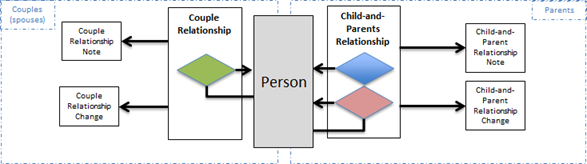
\includegraphics{05/04_relationshipsCore}
        \centering
        \caption{El bloc de l'arbre familiar relatiu a les relacions}\label{img:relationshipsBloc}
    \end{figure}

    Podreu observar també, a les taules que representen l'estructura dels recursos, que a vegades, per la columna que marca el format de dades d'un paràmetre, aquest es troba especificat entre els caràcters `[' i `]'. Aquesta terminologia s'utilitza per indicar que aquest paràmetre és en realitat un recurs o objecte de dades diferent inclòs dins del recurs estudiat.

    També s'observarà que sovint, els recursos exposats, hereten dades d'altres recursos i en els casos que aquests siguin rellevants, se n'exposarà l'estructura a l'apartat `Altres recursos interessants', més endavant en la memòria.

    \subsection{El recurs Relació (Relationship)}

    \paragraph{}
    Aquest recurs s'utilitza en l'actualitat per representar només les relacions de parella. En el passat, també va ser utilitzat per representar relacions entre pares i fills, mitjançant l'ús del paràmetre \emph{type} i l'enumeració \emph{relationshipType}. Tanmateix, aquest ha caigut en el desús des de la incorporació del recurs Relacions Pares i Fill.

    Aquest recurs emmagatzema informació sobre les persones que conformen la relació i els esdeveniments relacionats a aquesta. Les dades pròpies del recurs es mostren a la taula~\ref{res:relationship} i també hereta les dels recursos Subjecte, Conclusió, Enllaços Hypermedia i Dades Extensibles que poden ser trobats a l'apartat `Altres recursos interessants'.

    \begin{center}
             \csvreader[
                separator=comma,
                before table=\sffamily\small,
                longtable={p{2cm-2\tabcolsep}p{3.5cm-2\tabcolsep}p{8.5cm-2\tabcolsep}},
                table head={\caption{Paràmetres del recurs Relació}\label{res:relationship}\\\toprule%
                    \headentry{m{2cm-2\tabcolsep}}{Paràmetre}
                    & \headentry{m{3.4cm-2\tabcolsep}}{Format de Dades}
                    & \headentry{m{8.5cm-2\tabcolsep}}{Descripció}\\\midrule},
                late after line=\\\midrule,
                late after last line=\\\bottomrule,
             ]
             {./tables/05/02_relationships/relation.csv}
             {param=\param,format=\format,desc=\desc}
             {\param&\format&\desc}
     \end{center}


    \subsubsection{L'enumeració relationshipType}

    \paragraph{}
    L'enumeració relationshipType segueix l'estructura de definició GEDCOMX. Com a tal, els valors possibles per l'enumeració segueixen la pauta:\\\verb|http://gedcomx.org/ + `relationshipType'|

    La següent taula mostra els possibles valors per l'enumeració relationshipType, però com ja hem comentat, l'ús del valor ParentChild, ja no s'utilitza en favor del nou recurs Relació Pares i Fill.

    \begin{center}
        \csvreader[
           no head,
           separator=comma,
           table head={\caption{Valors possibles per l'enumeració relationshipType}\label{rel:relationshipType}},
           before table=\sffamily\small,
           longtable={|p{3cm}|p{3cm}|},
           column count=4,
           late after head=\\\hline,
           late after line=\\\hline,
           late after last line=\\\hline,
        ]
        {./tables/05/02_relationships/relationshipType.csv}
        {1=\one,2=\two}
        {\one&\two}
    \end{center}

    \subsection{El recurs Relació Pares i Fill (ChildAndParentsRelationship)}

    \paragraph{}
    Com ja hem comentat, aquest recurs s'utilitza per representar les relacions entre dos pares i un fill. Existeix també la possibilitat de deixar un pare sense especificar, permetent així, la introducció de famílies monoparentals en el sistema.

    Aquest recurs conté informació sobre les persones que conformen els rols de pare, mare i fill, així com el conjunt d'esdeveniments relacionats amb el pare i la mare.

    Els paràmetres del recurs són descrits sa la taula~\ref{res:childAndParents} i recordar que també hereta els paràmetres dels recursos Subjecte, Conclusió, Enllaços Hypermedia i Dades Extensibles que poden ser trobats a l'apartat `Altres recursos interessants'.

    \begin{center}
             \csvreader[
                separator=comma,
                before table=\sffamily\small,
                longtable={p{2cm-2\tabcolsep}p{3.5cm-2\tabcolsep}p{8.5cm-2\tabcolsep}},
                table head={\caption{Paràmetres del recurs Relació Pares i Fill}\label{res:childAndParents}\\\toprule%
                    \headentry{m{2cm-2\tabcolsep}}{Paràmetre}
                    & \headentry{m{3.4cm-2\tabcolsep}}{Format de Dades}
                    & \headentry{m{8.5cm-2\tabcolsep}}{Descripció}\\\midrule},
                late after line=\\\midrule,
                late after last line=\\\bottomrule,
             ]
             {./tables/05/02_relationships/parents.csv}
             {param=\param,format=\format,desc=\desc}
             {\param&\format&\desc}
     \end{center}

